
\chapter{Introduction\label{chpt:introduction}}

This thesis is about to develop an original numerical toolkit for
physical chemists and structural biologists, based on the molecular
density functional theory (\acs{MDFT}), which makes it possible to
predict efficiently, and with a microscopic accuracy, the solvation
properties of arbitrary molecular objects in arbitrary molecular solvents
(mainly water). This introduction will help to understand the objective
of this thesis, it explains why people are interested in the nature
of solvation, and where we are in the computing trends in solvation
simulation.


\section{Simulation of solvent effects}

Solvation is a fundamental phenomenon in chemistry. The chemical behavior
of lots of systems has a strong dependence on the nature of solvent.
For example, for some popular issue as metal-organic reacting center
\citep{Mn-oxo,PCET}, or pharmaceutical etudes \citep{drug_1_Perlovich,drug_2_Perlovich,drug_3}.
The solvation properties required by etudes are very variable, such
as the Gibbs free energy of solvation, solubility, partition coefficient,
saturated vapor pressure, pH value, as well as the 3D solvation structure,
etc. Overall, the interest of these solvation properties comes from
many domains, such as chemistry, biochemistry, pharmaceutics, medicine,
environmental and agrochemical industries. Unlike the well-studied
quantum mechanics (\acs{QM}) for chemical interaction and macroscopic
finite element model for physical process, the theories of solvation
are very variable and still under developing, owing to the ambiguous
compromise between the accuracy and the computing cost. In a word,
the studies in this domain are quite important and vibrant.

\begin{figure}[h]
\centering{}\textcolor{red}{}%
\begin{minipage}[t]{1\textwidth}%
\begin{center}
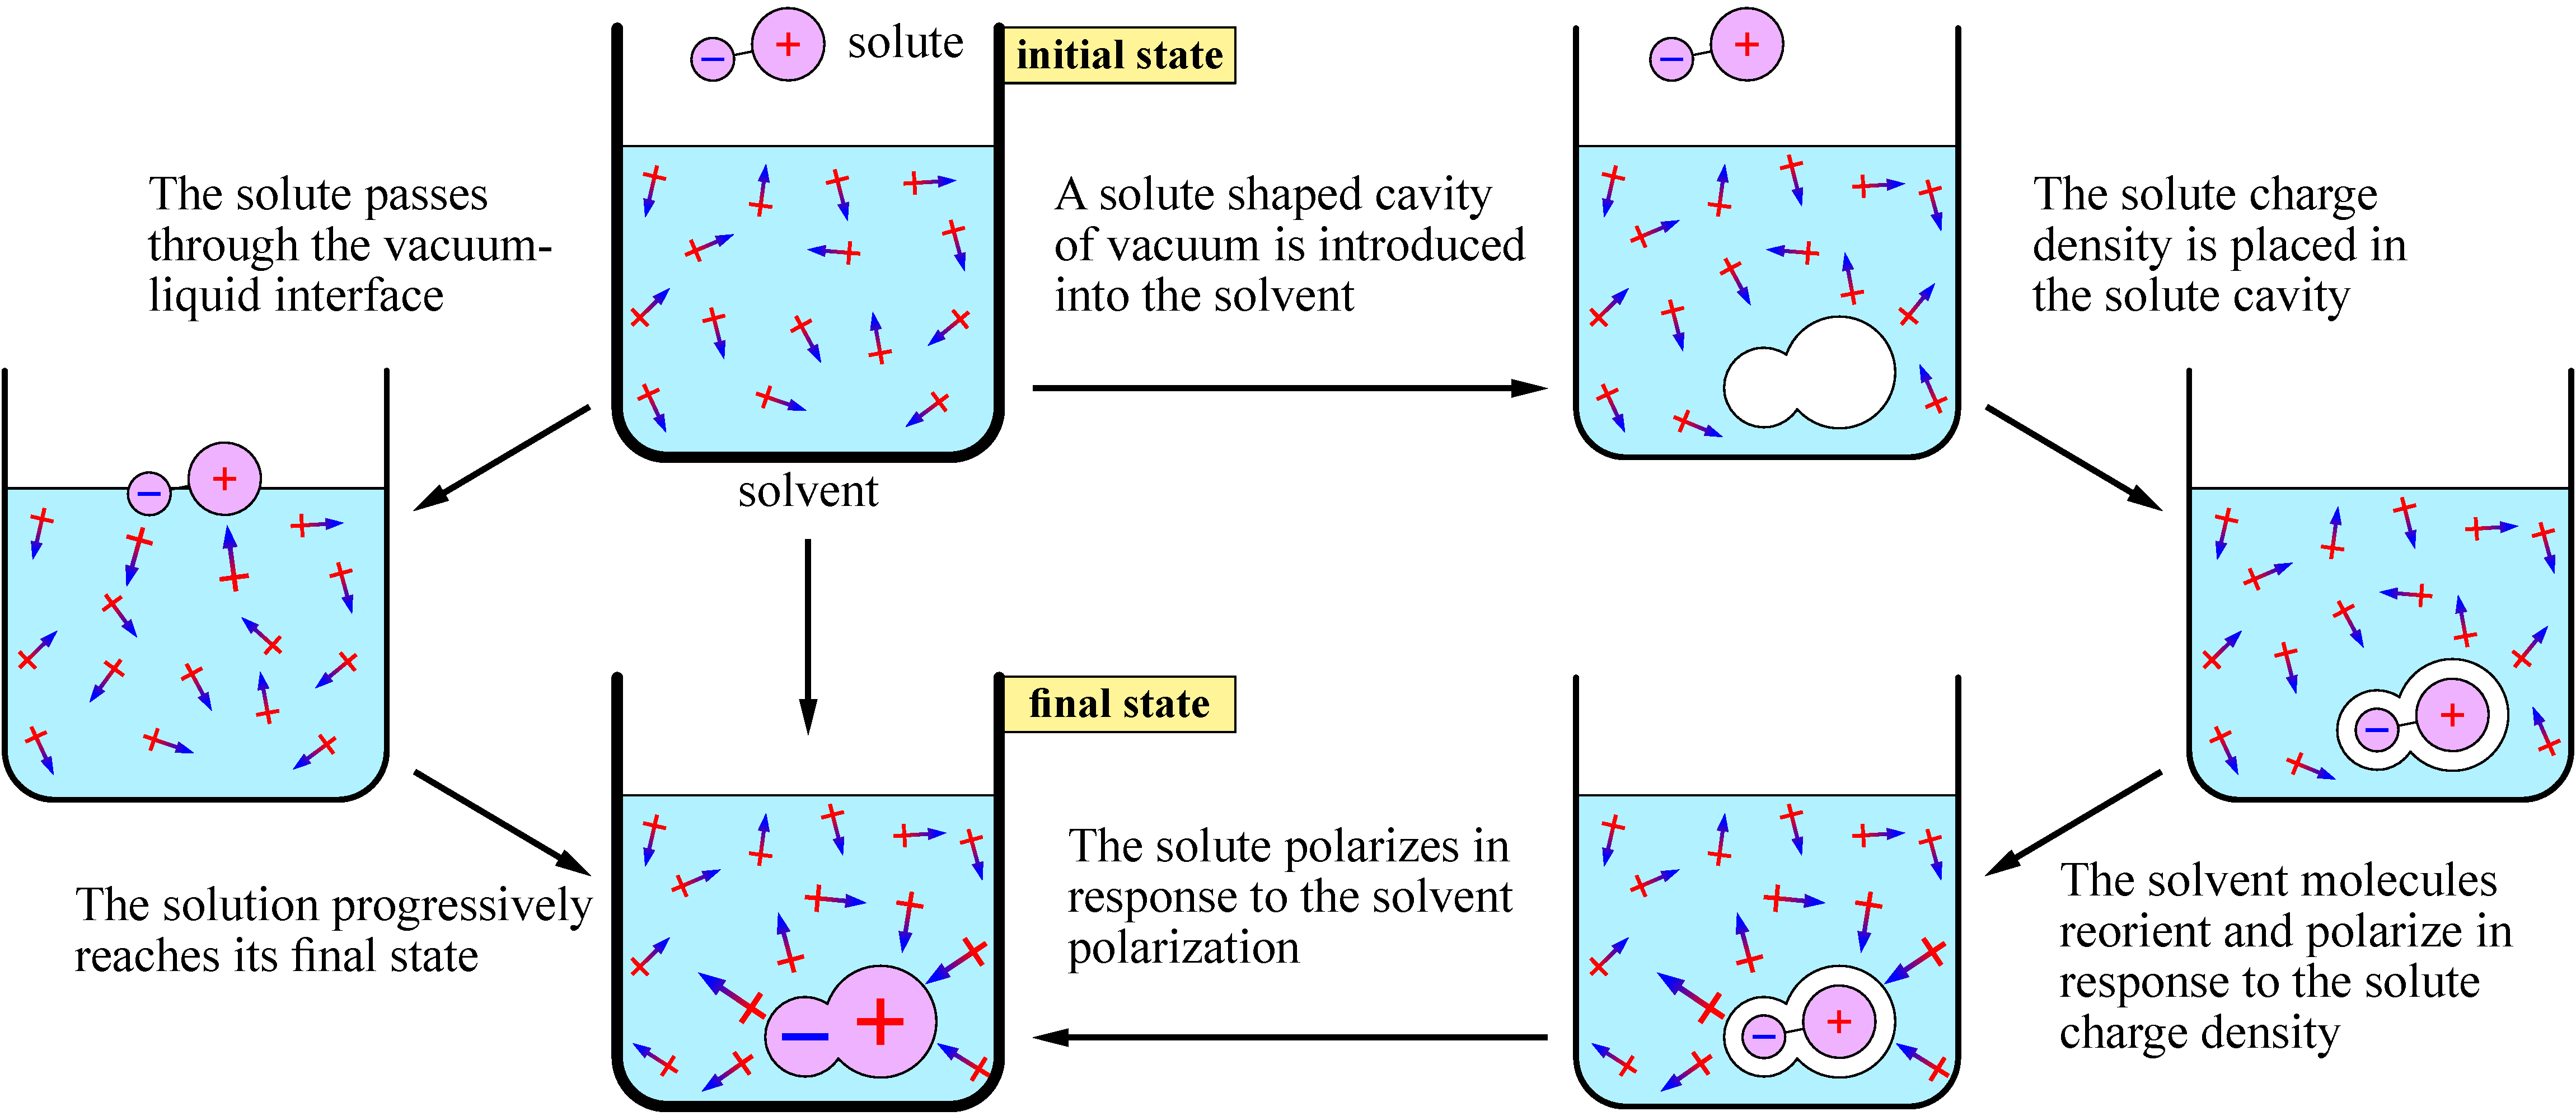
\includegraphics[width=1\columnwidth]{_figure/solvation}\caption[The solvation process]{The solvation process.\label{fig:Process-of-solvation} To a thermodynamic
system, whose properties only depends on the initial and final states,
it can go through different paths. The physical process of solvation
(left path)takes the solute from vacuum into bulk solvent, progressively
passing through the vacuum-liquid interface. Theoretically, the solvation
energy is defined as the energy consumed in such a progress. In theoretical
studies, the process can be decomposed to some artificial unphysical
process (right path), involving the growth of an uncharged solute-sized
cavity within the bulk solvent, the transfer of the solute charge
distribution from vacuum into the cavity, and the interaction between
the solute and solvent, etc.}

\par\end{center}%
\end{minipage}
\end{figure}


To change a phenomenon to a model, we must understand its process.
Solvation is defined as the process of moving a molecule from the
gas phase (or vacuum) to a condensed phase (figure \ref{fig:Process-of-solvation}),
which builds a stabilizing interaction with the solute (or solute
moiety like protein residues, interfaces, etc.) \citep{iupac}. Such
interactions are mostly classical, involving electrostatic forces
and van der Waals forces, with also chemically more specific effects
such as hydrogen bond formation, and quantic effects for some small
solvents whose vibrational or rotational energy states is at the same
magnitude as $k_{\mathrm{B}}T$, etc. \citep{Gray-Gubbins}.

As not all kinds of interactions is important in applications, according
to the usage, different models and methods are developed.

In the most of the 20th century \citep{Cramer_1999}, the study of
solvation effects has been dominated by continuum (implicit) models,
which is simply depending on the dielectric constants and not costly
on computation resource. They provide an accurate way to treat the
strong, long-range electrostatic interactions which dominate many
solvation phenomena, but lack of detail informations in the first
solvation shell. The later, which mainly includes the cavity formation
energy and solute-solvent van der Waals interactions, is often rudely
treat by introducing an artificial form of cavity, that links to the
form of solute. And the methods for electrostatic interactions involves
like generalized Born model, or through better estimates via Poisson-Boltzmann
calculations. They are widely integrated within \acs{QM} simulations
of the solvent, by add extra solvation terms onto the Fock or Kohn-Sham
operator \citep{Jensen,scrf,Tomasi_1994_implicit_model}. However,
the improper treatment of the first-shell, where the microscopic interactions
are primarily located, often introduce sometimes huge error in free
energy evaluation, especially for polar solvents (like water), despite
the accuracy that the \acs{QM} calculation alone can achieve. Therefore,
classical molecular simulations, which describing the individual solvent
molecules (explicit), particularly the molecular dynamics (\acs{MD})
and Monte Carlo method (\acs{MC}), became the alternative solution
during the last few decades. They generate trajectories and configurations,
then estimate free energy changes by statistical mechanic technics,
such as free energy perturbation (FEP) theory or thermodynamic integration
(TI) \citep{Jorgensen_1995_MC}. These calculation is very demanding
on computing cost, due to the requirement of many (hundreds or thousands
of) solvent molecules to form a realistic model.

Recently, a third domain of theory to describe solvent, based on the
statistical mechanics of fluid, is growing rapidly. It is generally
called liquid theory, involves mainly the integral equation theory
(\acs{IET}), and the classical density functional theory for liquids.
These approaches are cope to give the molecular nature of the first-shell,
but without calculate all the instantaneous micro-states with respect
to time, which can be integrated over positions and momentums theoretically.
Therefore, they are of magnitudes faster than those simulations by
micro-states.

The integral equation theory (\acs{IET}) is about solving the Ornstein-Zernike
(\acs{OZ}) equation with a specific closure equation \citep{Hensen-McDonald,Gray-Gubbins}.
It was firstly limited to so called ``simple liquid'' - a system
of spherical particles. A part, Chandler and Andersen in 1971 \citep{Chandler_1972_RISM}
developed the reference interaction site model (\acs{RISM}), which
discretizes the distribution and correlation functions into a site-site
set of functions, and solve the \acs{OZ} equation in matrix \citep{hirata_molecular_2004}.
Another part, Blum \citep{Blum_I,Blum_II}, Fries and Patey \citep{Fries_Patey_1985}
extend the \acs{OZ} equation to molecular case, where the distribution
and correlation functions depend on both position and orientation.
In their theory, the orientation part of \acs{OZ} equation is simplified
by expending the distribution and correlation functions on Wigner
generalized spherical harmonics.

The classical density functional theory approach deal with inhomogeneous
liquids, which uses the same variation principle and minimization
strategy \citep{mermin_thermal_1965,Evans_1979,Hansen_1987} as electronic
density functional theory \acs{DFT} that treats electric interactions
and has a great success in computational chemistry. It gives the Helmholtz
free energy and the equilibrium solvent density, by minimizing the
free energy functional of the solvent density in the presence of a
given external potential. Borgis and collaborators \textcolor{red}{{[}too
many ref{]}} have recently generalized it into molecular case, named
molecular density functional theory (\acs{MDFT}), where the solvent
density depends on both position and orientation, $\rho(\mathbf{r},\mathbf{\Omega})$.
The main theoretical difficulty lies in the definition of well-funded
and reliable functionals of the excess free energy $\mathcal{F}_{\mathrm{exc}}\left[\rho\right]$,
according to the geometric complexity of the solvent molecule. Some
recent researches have shown that it is cope with linear solvents
like acetonitrile, but still have little non-satisfaction with the
most complex solvent, i. e. water. \acs{MDFT} can be proved to be
mathematically equivalent to the two-component molecular \acs{IET}.

The majority of work of all these theories have been focused on water,
since it is one of the most difficult systems to model due to its
molecular geometry, ineligible multi-body interaction, quantum effect,
hydrogen bond, etc. The importance of including instantaneous polarization
in potential functions is also an issue \citep{polarisable_1,polarisable_2}.
However, since polarizable force fields are not yet in common use,
the simulations by micro-states and the liquid theory which feed on
force field also have their own limit, compared to the continuum model
which can be polarizable. The advantages and disadvantages of each
branch of theory are listed in table \ref{tab:Theories-of-solvation}.

\begin{table}[h]
\begin{centering}
\begin{tabular}{ccccc}
\toprule 
\tableheadline{Theory} & \tableheadline{Speed} & \tableheadline{Long-Range} & \tableheadline{First-Shell} & \tableheadline{Polarizable Solvent}\tabularnewline
\midrule
Continuum model & fast & yes & no & fully\tabularnewline
Simulation by time & costly & yes & yes & partially, very costly\tabularnewline
Liquid theory & fast & yes & yes & partially\tabularnewline
\bottomrule
\end{tabular}
\par\end{centering}

\caption{Theories of solvation simulation\label{tab:Theories-of-solvation}}
\end{table}


This thesis consists in the development of the \acs{MDFT}, focusing
on the generalization and algorithmic acceleration of the excess free
energy functional $\mathcal{F}_{\mathrm{exc}}$ evaluation under homogenous
reference fluid (\acs{HRF}) approximation, which will be discussed
in detail in later chapters. 


\section{Scope of this thesis}

Chapter I reviews a selection of models and methods to the solvent
effect. It includes the mainly used continuum model, the basic of
liquid theory, as well as its two frontier research domains, \acs{IET}
and \acs{MDFT}. The code structure of \acs{MDFT}, which all the
development in this thesis is based on, is also presented. There is
also a brief introduction to \acs{MD} and \acs{MC}, as well as the
generation of direct correlation function (\acs{DCF}) used in this
thesis by such methods. 

Chapter II presents all the theory developed and newly used in this
thesis. In this thesis, two algorithms of excess energy functional
evaluation are proposed, one is extension of the previous algorithm,
other is a new algorithm, that combines the molecular \acs{OZ} equation
treatment of angular part with MDFT. The output solvation properties
is mainly the two: free energy, and solvent structure.

Chapter III takes note of all the implementation result, that divided
into two aspects, the ``accuracy'', which involves comparisons between
algorithms, and with \acs{IET} and \acs{MD} results; and the ``efficiency'',
which evaluate the computing cost of the code, both in sequential
and parallelized version.

Chapter VI gives some application to ions and molecules.
